\section{Command}

O padrão Command permite encapsular operações 
em objetos. Isso permite que seja mantido um 
histórico das operações realizadas, que seja 
criada uma sequência de operações a serem 
executadas e até mesmo que operações realizadas 
possam ser desfeitas.\cite{gamma:1995}

Para alcançar isso, uma classe Command armazena o 
objeto alvo da operação e define uma operação 
de execução e uma de reversão, quando necessário. 
Uma outra classe pode ser responsável por armazenar 
uma coleção de \textit{commands}, mantendo o 
histórico ou sequência de operações. 

Esse padrão funciona como uma solução para definir 
\textit{callbacks}, ou seja, operações que podem ser 
predefinidas e executadas futuramente no código. Sua 
estrutura pode ser vista na imagem \ref{command_struct}.

\begin{figure}[htb]
	\caption{\label{command_struct}Estrutura do Command}
	\begin{center}
	    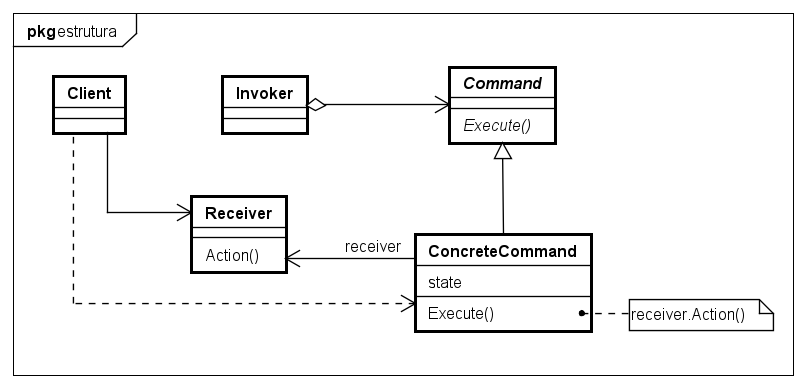
\includegraphics[scale=0.5]{5_padroes-contexto-funcional/5.3_comportamentais/5.3.02_command/command_struct.png}
	\end{center}
\end{figure}

\subsection*{Exemplo Orientado a Objetos}

O exemplo do Command traz um \textit{toolkit} para 
construção de interfaces de usuário, onde ao clicar 
ou realizar uma ação sobre botões e menus, uma 
operação deve ser executada. Porém, os botões e 
menus não devem conhecer essas operações, elas são 
definidas pelo desenvolvedor que utiliza os toolkits. 
Dessa forma, o padrão Command permite isolar as 
operações dos \textit{widgets}. O exemplo traz as 
operações PasteCommand, que tem como alvo um 
documento da aplicação, e OpenCommand, que tem como 
alvo o objeto da aplicação. Além disso, há um 
MacroCommand que permite executar uma sequência 
de comandos. O exemplo é apresentado no diagrama da 
imagem \ref{command_exemplo} e no código \ref{oocommand}.

\begin{figure}[htb]
	\caption{\label{command_exemplo}Exemplo de Command}
	\begin{center}
	    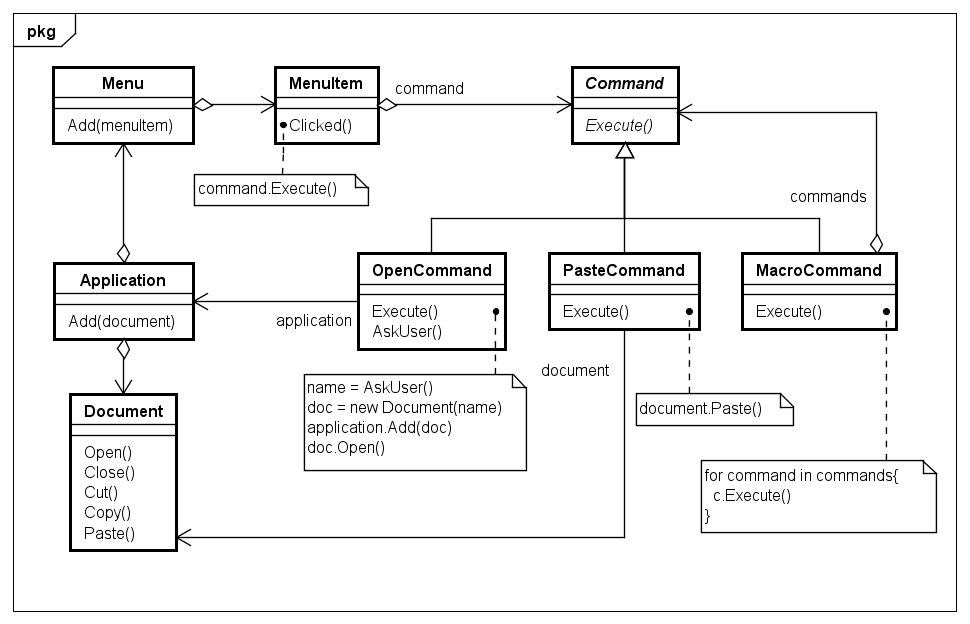
\includegraphics[scale=0.5]{5_padroes-contexto-funcional/5.3_comportamentais/5.3.02_command/command_exemplo.png}
	\end{center}
\end{figure}

\begin{lstlisting}[caption={Command Orientação a Objetos},label=oocommand]

abstract class Command {
  def Execute()
}

class OpenCommand(var application : Application) extends Command {
  def Execute(): Unit = {
    var name = AskUser()
    if(name != null){
      val document = new Document(name)
      application.Add(document)
      document.Open()
    }
  }

  def AskUser() : String = {
    //Solicita ao usuário o arquivo que será aberto
  }
}

class PasteCommand(var document : Document) extends Command {
  def Execute(): Unit = {
    document.Paste()
  }
}

class MacroCommand extends Command {

  private var commands : List[Command] = List()

  def Execute(): Unit = {
    commands.foreach(command => {
      command.Execute()
    })
  }
}
    
\end{lstlisting}

\subsection*{Contexto Funcional}

A a intenção do Command é encapsular operações 
em objetos. Isso já é possível no contexto 
funcional graças às funções de alta ordem. 
Entretanto, existem duas particularidades 
do padrão Command que devem ser consideradas. 

O padrão encapsula, junto da operação, uma 
referência para o objeto alvo. Dessa forma, 
quando a operação é realizada, ocorre 
um efeito colateral, desencorajado 
no contexto funcional. Para evitar isso, o 
comando deve receber, ao ser executado, o 
valor alvo como parâmetro e retornar o 
valor atualizado.

A segunda particularidade é que o padrão 
também permite uma operação de desfazer. Como 
tanto a operação de fazer quanto a de desfazer 
são encapsuladas em um mesmo objeto, é necessário 
definir um valor, como uma tupla, que armazene ambas 
as operações.

O código \ref{fpcommand} demonstra uma implementação 
genérica do padrão no contexto funcional. Na linha 2 
é definido um tipo Command que é uma tupla que 
armazena duas funções: fazer e desfazer. A função 
CreateCommand, na linha 4, é uma função auxiliar para 
a criação de um command. Caso não seja fornecida 
uma função de desfazer, a função é substituída por 
uma função identidade que recebe um valor como 
parâmetro e retorna esse mesmo valor.

As funções auxiliares Execute, na linha 12, e 
Unexecute, na linha 14, recebem como parâmetro o valor 
alvo e um comando. Elas executam a primeira e a 
segunda função armazenadas na tupla Command, 
respectivamente. A função CommandMany, da linha 16, 
é uma função auxiliar 
para executar uma lista de \textit{commands}. Ela recebe 
como parâmetro um alvo, uma lista de \textit{commands} e 
uma operação que recebe um alvo e um comando. Essa 
operação genérica é utilizada para que essa função 
possa ser reaproveitada tanto para executar uma 
sequência de \textit{commands} quando desfazê-los. 
As funções ExecuteMany, na linha 20, e UnexecuteMany, 
na linha 23, chamam a função CommandMany passando 
como operação as função Execute e Unexecute, 
respectivamente.


\begin{lstlisting}[caption={Command Funcional},label=fpcommand]
    
type Command[A] = (A => A, A => A)

def CreateCommand[A](Do : (A) => A,
                     Undo : Option[(A) => A] = None) : Command[A] =
  (Do,
    Undo match {
      case Some(function) => function
      case None => (x) => x
  })

def Execute[A](target : A, command : Command[A]) : A = command._1(target)

def Unexecute[A](target : A, command: Command[A]) : A = command._2(target)

def CommandMany[A](target : A, commands : List[Command[A]], operation : (A, Command[A]) => A): A =
    if(commands.isEmpty) target
    else CommandMany(operation(target, commands.head), commands.tail, operation)

  def ExecuteMany[A](target : A, commands : List[Command[A]]) : A =
    CommandMany(target, commands, Execute)

  def UnexecuteMany[A](target : A, commands : List[Command[A]]) : A = {
    CommandMany(target, commands, Unexecute)
    
\end{lstlisting}

O código \ref{fpcommandexample} demonstra como o exemplo 
orientado a objetos poderia ser implementado a partir das 
funções auxiliares vistas. O valor ExecuteOpen, visto 
na linha 2, implementa a abertura de um documento em uma 
aplicação e retorna o estado atualizado dessa aplicação 
com o documento aberto. Já a função ExecutePaste, na 
linha 8, realiza a operação de colar um documento. 
O valor resultingApplication na linha 14 é o estado 
resultante da aplicação após a execução de ambos os 
comandos através da função auxiliar ExecuteMany.

\begin{lstlisting}[caption={Exemplo funcional de Command},label=fpcommandexample]
    
val ExecuteOpen = CreateCommand[Application](
  (target : Application) => {
    //Executa comando de abrir
  } : Application
)

val ExecutePaste = CreateCommand[Application](
  (target : Application) => {
    //Executa comando de colar
  }
)
  
val resultingApplication = ExecuteMany(application, List(ExecuteOpen, ExecutePaste))
    
\end{lstlisting}

\begin{comment}
\subsection*{Vantagens e Desvantagens}

O Command funcional consegue economizar classes, resumindo a 
complexidade do padrão à criação de uma tupla para os casos 
onde é desejado implementar a operação de desfazer. Para 
os casos onde isso não é necessário, a implementação se torna 
ainda mais simples, já que as funções de alta ordem em si 
já suprem a necessidade de encapsular operações. A grande 
desvantagem da implementação funcional é que a execução das 
operações se torna mais dependente do valor alvo. O valor 
atualizado sempre precisa ser repassado para o comando para 
que qualquer modificação feita anteriormente - seja por outro 
trecho da aplicação ou por um comando executado anteriormente - 
seja considerada durante a execução.
\end{comment}